% !TeX root = ../main.tex

\chapter{索引模块的实现}

之前的章节中我们着重介绍了如何设计索引的各个组成部分,接下来的一章中,我们将探讨如何实现这一索引.

\section{索引节点的底层存储实现}

以下定义索引节点的结构体,如图所示所有类型的索引节点都包含一个仅有头部数据的节点类Node。

\begin{figure}[h]
  \centering
  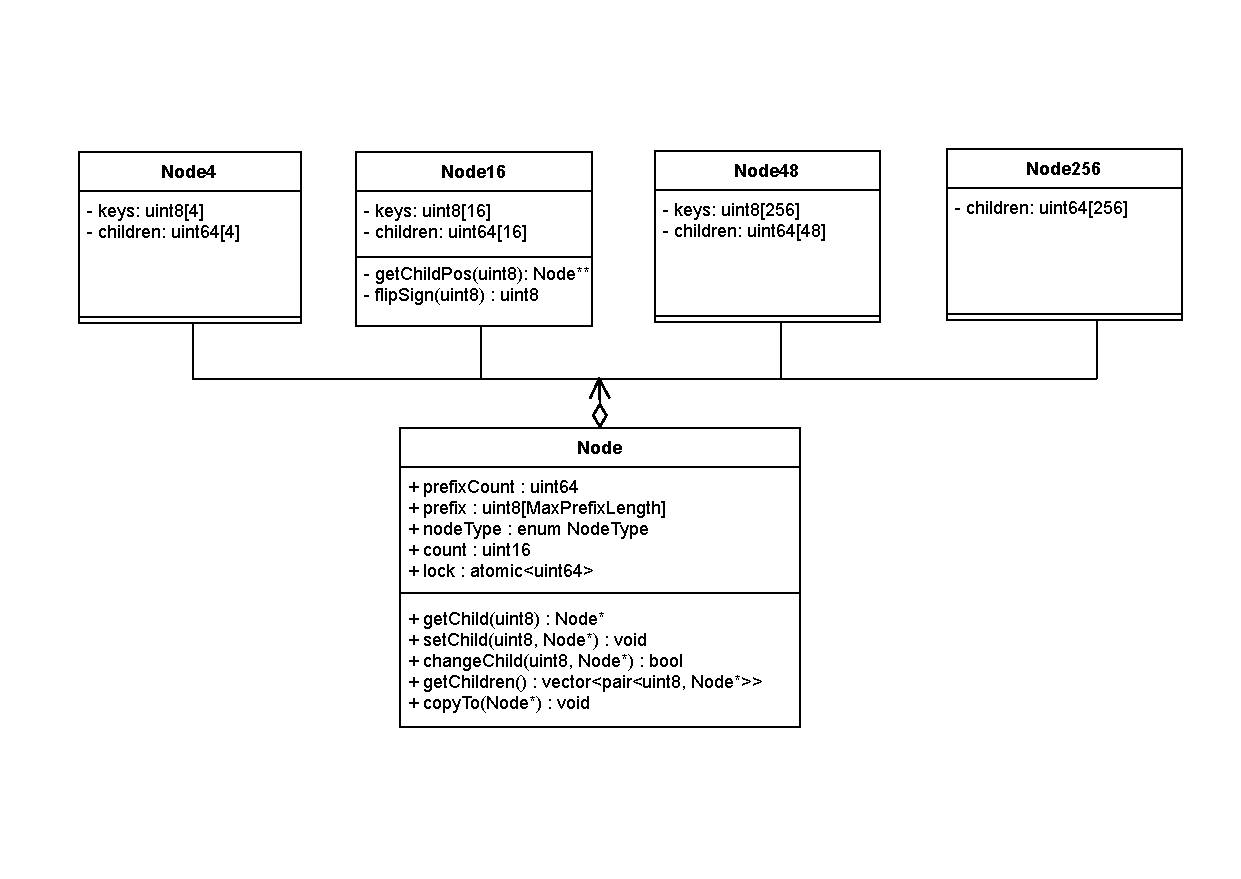
\includegraphics[width=1\textwidth]{ART-node-class.pdf}
  \caption{ART索引节点的类图}
  \label{fig:ART-node-class}
\end{figure}

\textbf{Node :}
\begin{itemize}
\item prefixCount : 公共前缀的长度,uint64类型

\item prefix[MaxPrefixLength] : 公共前缀,长度为MaxPrefixLength的字符串

\item nodeType : 节点的实际类型,enum {Node4, Node16, Node48, Node256} 类型

\item count : 节点中实际存储的子节点个数,uint16类型

\item lock : 前文中提到的乐观锁,std::atmoic<uint64>类型

\item getChild(): 返回key对应的孩子节点

\item setChild(): 设置某个孩子节点的指针,并将节点中子节点个数加1

\item changeChild(): 设置某个孩子节点的指针

\item getChildren(): 获得该节点的所有非空的孩子节点指针 
\end{itemize}

\textbf{Node4:}
\begin{itemize}
\item keys[4] : 子节点的键值,uint8类型数组

\item children[4] : 指向子节点的指针,uint64类型数组
\end{itemize}

\textbf{Node16:}
\begin{itemize}
\item keys[16] : 子节点的键值的补码,uint8类型数组

\item children[16] : 指向子节点的指针,uint64类型数组
\end{itemize}

\textbf{Node48:}
\begin{itemize}
\item keys[256] : keys[i]存储键值为i的子节点的在children数组中的索引,uint8类型数组

\item children[48] : 指向子节点的指针,为uint64类型数组
\end{itemize}

\textbf{Node256:}
\begin{itemize}
\item children[256] : 指向子节点的指针,uint64类型数组
\end{itemize}

以上为节点的私有的成员变量介绍,除此之外,节点还需要实现一些公共的方法,方便上层函数进行相关调用。这些接口包括getChild,setChild,changeChild,copyTo等。 
我们这里在基类中实现的是静态方法,在每种类型的子类节点都需要实现相应的方法。之后在父类中根据不同的
节点类型(前文中描述的NodeType)调用对应对象的方法。

针对不同的节点类型做的优化方法的实现:首先每一种类型的节点其内部的键值都是有序的,这一点是为了方便后续的范围查询。对于子节点数量最少的
Node4类型,按顺序查询相应的child即可,但是对于Node16类型,如果是循环查询对应的child,至多需要查询15次,效率明显下降,因此对于Node16类型的节点。
我们利用SIMD加速,一次操作128字节的keys。具体实现方法如下。

\begin{lstlisting} 
N *const *GetChildPos(const uint8_t k) const {
    __m128i cmp = _mm_cmpeq_epi8(_mm_set1_epi8(flipSign(k)),
        _mm_loadu_si128(reinterpret_cast<const __m128i *>(keys)));
    unsigned bitfield = _mm_movemask_epi8(cmp) & ((1 << count) - 1);
    if (bitfield) {
        return &children[ctz(bitfield)];
    } else {
        return nullptr;
    }
}

void SetChild(const uint8_t k, N *child) {
    uint8_t keyByteFlipped = flipSign(k);
    __m128i cmp = _mm_cmplt_epi8(_mm_set1_epi8(keyByteFlipped),
        _mm_loadu_si128(reinterpret_cast<__m128i *>(keys)));
    uint16_t bitfield = _mm_movemask_epi8(cmp) & (0xFFFF >> (16 - count));
    unsigned pos = bitfield ? ctz(bitfield) : count;
    memmove(keys + pos + 1, keys + pos, count - pos);
    memmove(children + pos + 1, children + pos, 
            (count - pos) * sizeof(N *));
    keys[pos] = keyByteFlipped;
    children[pos] = child;
    count++;
}
\end{lstlisting}

我们主要使用的是C++标准库中对SSE指令集的封装,\_mm\_cmplt\_epi8和\_mm\_cmpeq\_epi8分别支持对128bit的数据比较大小。前提是128bit其中存储的16个有符号数,
因此这里我们需要做一个转换flipSign(k)将传入的无符号k转换,便于使用有符号的SSE指令比较无符号数的大小。
\_mm\_cmplt\_epi8指的是两个128bit数每8bit比较大小,返回128bit的结果,其中每8bit为对应的两个8bit比较出的结果,返回1表示小于成立,否则返回0.
\_mm\_movemask\_epi8将结果转换为16bit的整型,ctz主要是计算实际的比较的结果中末尾存在0的个数。并根据此计算出应该将对应的k插入到具体的位置。

对于GetChildPos接口,主要是被getChild等查询子节点的函数调用,原理类似与上面setChild,但是SIMD指令稍有不同,这里是查询对应的k在索引节点中是否存在因此
选取的就是\_mm\_cmpeq\_epi8指令,比较的是对应的位置上是否有8bit的数据也就是key与目标key相同,若有相同返回1,没有相同则返回全0。
随后\_mm\_movemask\_epi8将结果转换为16bit的整型,再与((1 << count) - 1)相与,判断是否有k满足条件。

对于Node48,则是存储了256个key和48个槽位。每一个key中存储的都是对应槽位的索引,因此仅需要将无效的槽位标记为48。有效槽位的索引不可能大于48。
由此来降低在每个索引内部节点查询下层子节点的开销。

对于Node256,则是最基本的前缀树存储,只存储对应的256个指向子节点的指针,我们只需要通过的键值中对应位置的byte作为索引即可获得对应的子节点指针。
 
以上是在实现每一种Node节点类型时在工程上作出的优化,通过利用SIMD等操作,大大降低节点插入和查询的开销。对于Node48,通过在keys数组中
存储children数组索引的方式,用空间换取时间,也可以降低查询的开销。
\section{索引乐观锁实现}

上面提到的索引节点结构中,lock即为索引节点的乐观锁实现。以下为Node基类中关于lock的通用接口。

\begin{itemize}

\item ReadlockOrRestart(): 获得当前节点的读锁,若写标记或删除标记为1,则restart;否则返回当前的版本号

\item writeLockOrRestart(): 获得当前节点的写锁,若写标记或删除标记为1,则restart;否则版本增加1

\item upgradeLockOrRestart(): 将当前的读锁升级为写锁,若与读锁的版本号不一致,则restart;否则版本增加1

\item ReadUnlock(): 释放读锁,即比较当前版本号与先前版本号,若一致,返回成功;不一致,则restart

\item writeUnlock(): 释放写锁,即将当前节点的版本号加一

\item writeUnlockObsolete(): 释放写锁,并将节点标记为删除

\end{itemize}

以上对节点的锁的通用接口都被认为是具备原子性的。所有的对lock的修改操作都是通过c++中针对原子变量的操作
如lock.compare\_exchange\_strong()或者lock.fetch\_add()等。此外我们还需要设计使线程挂起的接口。
前文中提到当操作线程一直重启时,需要使线程挂起,等待系统冲突降低时,再执行该任务。
这里只需要使用系统中sched\_yield()调用,表示放弃当前的CPU即可。上面接口中的restart表示,当线程想要获得
锁被其他线程持有,或者是在获得锁到释放锁期间,有其他线程修改过锁时,该线程都会放弃这次操作,回到索引的
根节点重新开始一次操作。这在实现时可以使用一个goto语句实现。

\section{索引的并发控制机制}

\begin{figure}[h]
  \centering
  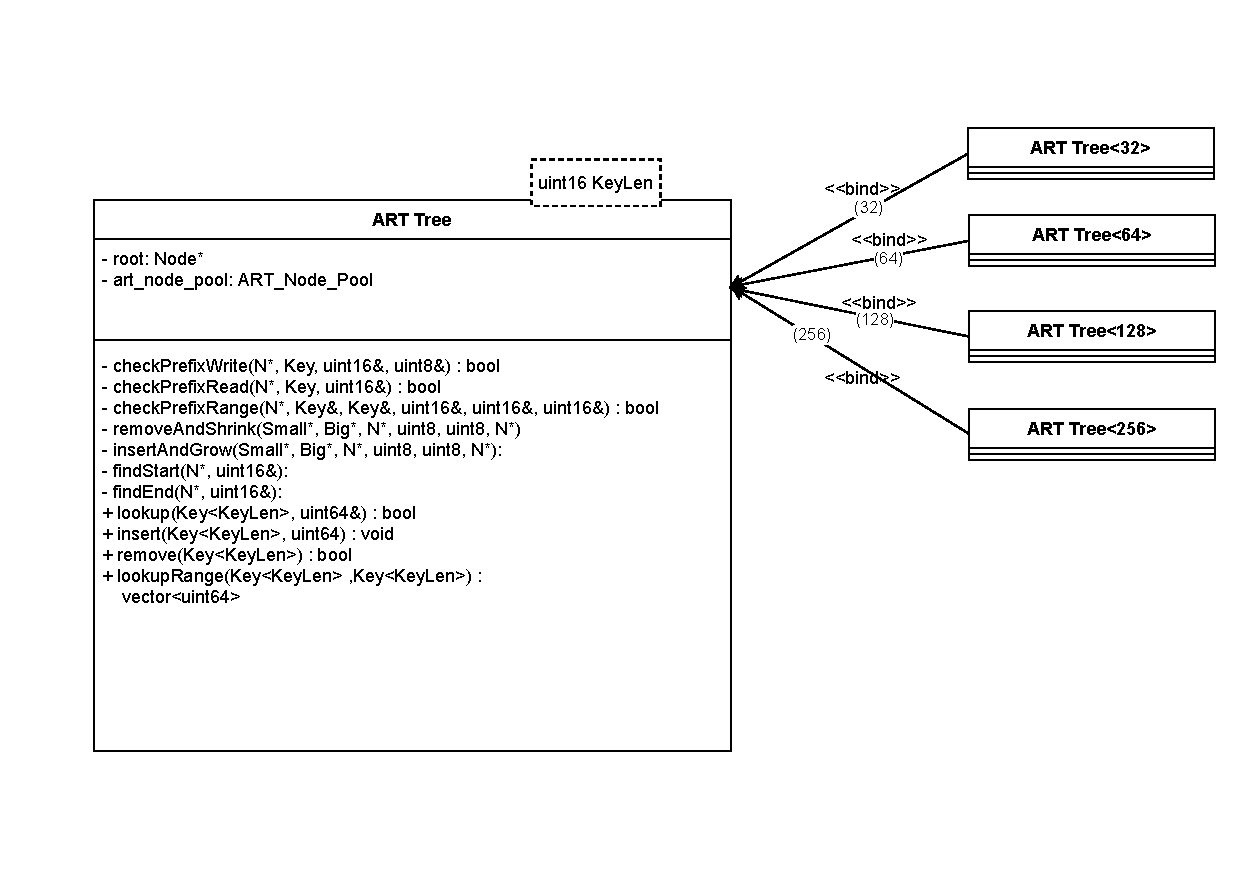
\includegraphics[width=1\textwidth]{ART-tree-class.pdf}
  \caption{ART Tree的类图}
  \label{fig:ART-tree-class}
\end{figure}

这一小节我们将介绍如何基于以上提到的数据结构和算法,实现ART索引的并发控制,对于ART来说主要需要实现以下几个public接口。
此外还需要实现针对内部结构的私有成员函数

\begin{itemize}

\item lookup(): 获得当前节点的读锁,若写标记或删除标记为1,则restart;否则返回当前的版本号

\item lookupRange(): 获得当前节点的写锁,若写标记或删除标记为1,则restart;否则版本增加1

\item insert(): 将当前的读锁升级为写锁,若与读锁的版本号不一致,则restart;否则版本增加1

\item delete(): 释放读锁,即比较当前版本号与先前版本号,若一致,返回成功;不一致,则restart

\end{itemize}

除了以上的公共的接口,索引还需要提供以下的私有函数,主要是为了解决节点伸缩问题以及处理不同类型操作中,
使用不同的前缀比较函数接口。


\begin{itemize}

\item removeAndShrink(): 删除对应的子节点的key和对应的孩子节点指针,并将当前节点缩容为更小的节点类型。
通过copyTo接口将剩下的keys和children拷贝到缩容后的新节点上。
同时修改父亲节点中对应的子节点指针,并将缩容前的节点做标记删除处理

\item insertAndGrow(): 申请节点容量更大的新节点,
通过copyTo接口将当前节点的keys和children拷贝到扩容后的新节点上。
插入对应的子节点的key和对应的孩子节点指针,
同时修改父亲节点中对应的子节点指针,并将扩容前的节点做标记删除处理

\item checkPrefixRead(): 对应查询/删除操作时的比较前缀的函数,当前缀不相等时,返回false,前缀相同的时候返回true

\item checkPrefixWrite(): 对应插入操作时的前缀比较函数,前缀不相等时返回false,同时也会返回不相等的key,以及相等部分的长度
前缀完全匹配时返回true

\item findStart(): 针对范围查询的辅助函数,差摘查找对应的上边界中是否有满足条件的结果,并返回结果集。

\item findEnd(): 针对范围查询的辅助函数,差摘查找对应的下边界中是否有满足条件的结果,并返回结果集。

\item checkPrefixRange(): 对应范围查询时,比较前缀与实际搜索的key的大小关系,若当前前缀在范围查询的[begin, end]之间
返回true,并且返回一个封闭区间[startKey, endKey],表示满足条件的区间查询的结果。针对上下边界可以使用上述的两个辅助函数进行
递归查询。最后合并 findStart(startKey), findEnd(endKey)以及(startKey, endKey)开区间上所有叶子节点。

\end{itemize}

以上分别介绍了索引实际操作的算法的接口下面我结合伪代码详细解释操作算法的实现过程。

\subsection{查询操作的实现}
对于ART索引来说,查询操作是一个最常用的操作,也是较为简单的一个操作,在查询操作中不涉及节点类型的变更,
也不涉及索引结构的修改。查询只需要从根节点开始,向下查询。每次进入当前节点时读取版本号,随后比较前缀,
若匹配进入下一层节点。在此之前,比较版本号是否存在变更。如此不断向下搜索直至找到对应的叶子节点。最后如果对应的
槽位上不含有指向子节点的指针,则返回Null。

\begin{breakablealgorithm} 
\counterwithin{algorithm}{chapter}
    \caption{ART索引查询流程伪代码} 
    \begin{algorithmic}[1]
    \begin{footnotesize}
    \hspace*{\algorithmicindent} \textbf{Input}{: key}\\
    \hspace*{\algorithmicindent} \textbf{Output}{: tid}
    \STATE {$cur \leftarrow root$}
    \STATE {$parent \leftarrow null$}
    \STATE {$level \leftarrow 1$}
    \WHILE{$level < KeyLen(key) $} 
        \STATE {$ReadLock(cur, v, needRestart)$}
        \STATE {$nextLevel \leftarrow level$}

        \IF{$checkPrefixRead(cur, key, level)$} 
            \STATE {$parent \leftarrow cur$}
            \STATE {$cur \leftarrow GetChild(cur, key[level])$}
            \STATE {$ReadCheck(parent, v, needRestart)$}

            \IF {$cur = null$} 
                \RETURN {false}
            \ENDIF

            \IF {$IsLeaf(cur) \And level = KeyLen(key)$}
                \STATE {$ReadUnlock(parent, v, needRestart)$}
                \STATE {$tid \leftarrow GetLeaf(cur)$}
                \RETURN {true}
            \ENDIF
        \ELSE 
            \STATE {$ReadUnlock(cur, v, needRestart)$}
            \RETURN {false}
        \ENDIF
        \STATE {$level \leftarrow level + 1$}
        \STATE {$ReadUnlock(cur, v, needRestart)$}
    \ENDWHILE
    \end{footnotesize}
    \end{algorithmic}
\end{breakablealgorithm}

\subsection{插入操作的实现}
索引的插入操作与查询操作最大的不同在于,前缀比较时,若不一致,则需要分裂当前节点,抽出最长的公共前缀。
此外,插入节点时可能会导致节点的扩容成容量更多的节点。整体的插入流程如下:从根节点开始,向下搜索,匹配
前缀,若不一致,申请新的Node4类型的节点,将公共前缀放入新申请的节点中,并且为新插入的key申请新的节点,
将curNode和nextNode插入newNode中,完成本次插入。若前缀一致,则需要查找对应的槽位是否有空缺,若不存在
子节点,则将nextNode插入对应的槽位,否则继续向下搜索,重复以上过程,直至节点可以被插入树中。

这里有个地方需要注意,实际我们编写代码时,没有使用路径压缩机制,实际如果我们使用路径压缩方式,不管是
查询还是插入,如果是采用路径压缩方式,则需要根据TID到数据库表中读取相应的字段,最后将各个字段组合成完整的
key,与需要比较的键值进行比较,这一步在内存数据库中,需要经过多次的访存,由于底层存储格式为行列混存。与一般
的行存不同,会导致读取多个字段的过程Cache是失效的。无法有效的利用CPU的Cache。而且,如果ART索引存储
的键值的长度都不会超长,每个节点的头节点部分存储着公共前缀。所以实际的树高是有限的,与多次访问
内存的开销相比也是可以忽略的。若树的节点都较为密集,而不是稀疏的存储一些值。那么压缩带来的优势也会大大降低。 
因此综上所述,我们并没有在实际实现时加入路径压缩,而是在路径上存储完整的键值。


\begin{breakablealgorithm} 
\counterwithin{algorithm}{chapter}
    \caption{ART索引插入流程伪代码} 
    \begin{algorithmic}[1]
    \begin{footnotesize}
    \hspace*{\algorithmicindent} \textbf{Input}{: key, tid}\\
    \hspace*{\algorithmicindent} \textbf{Output}{: void}
    \STATE {$cur \leftarrow null$} 
    \STATE {$next \leftarrow root$} 
    \STATE {$level \leftarrow 1$} 
    \WHILE{$level < KeyLen(key) $}
        \STATE {$parent \leftarrow cur$}
        \STATE {$cur \leftarrow next$}
        \STATE {$ReadLock(cur, v, needRestart)$}
        \STATE {$nextLevel \leftarrow level$}

        \IF{$!checkPrefixWrite(cur, key, nextLevel, noMatchKey, rePrefix, reLen)$} 
            \STATE // Prefix is not matched, split current Node
            \STATE {$CouplingLock(cur, parent, pv, v, needRestart)$}
            \STATE {$newNode \leftarrow new Node4()$}
            \STATE {$nextNode \leftarrow GenNewNode(key, nextLevel + 1, tid)$}
            \STATE {$newNode.SetPrefix(cur.GetPrefix(), nextLevel - level)$}
            \STATE {$cur.SetPrefix(remainPrefix, remainLen)$}

            \STATE {$SetChild(newNode, noMatchKey, cur)$}
            \STATE {$SetChild(newNode, key[nextLevel], nextNode)$}
            \STATE {$ChangeChild(parent, pk, newNode)$}

            \STATE {$WriteUnlock(cur)$}
            \STATE {$WriteUnlock(parent)$} 
        \ENDIF
        \STATE {$k \leftarrow key[nextLevel]$}
        \IF{$!GetChild(cur, k)$} 
            \STATE // current child pointer is null
            \IF{$cur.IsFull()$}
                \STATE // current node is full, should grow to bigger one.
                \STATE {$CouplingLock(cur, parent, pv, v, needRestart)$}
                \STATE {$InsertAndGrow(cur, parent, pk, k, GenNewNode(key, nextLevel + 1, tid))$}
                \STATE {$DeleteUnlock(cur)$}
                \STATE {$WriteUnlock(parent)$}
                \STATE {$markNodeForDeletion(cur)$}
            \ELSE 
                \STATE // current node is not full, insert tid into current node.
                \STATE {$UpgradeLock(cur, v, needRestart)$}
                \STATE {$SetChild(cur, k, GenNewNode(key, nextLevel + 1, tid))$}
                \STATE {$WriteUnlock(cur)$}
            \RETURN {}
            \ENDIF
        \ELSE
            \STATE {$next \leftarrow GetChild(cur, k)$}

            \IF{$IsLeaf(next)$}
                \STATE // The same Key is thought as update
                \STATE {$UpgradeLock(cur, v, needRestart)$}
                \STATE {$ChangeChild(cur, k, tid)$}
                \STATE {$WriteUnlock(cur)$}
                \RETURN {}
            \ENDIF

            \IF{$parent != null$} 
                \STATE {$ReadUnlock(parent, pv, needRestart)$}
            \ENDIF
        \ENDIF
        
        \STATE {$level \leftarrow nextLevel + 1$}
    \ENDWHILE
    \end{footnotesize}
    \end{algorithmic}
\end{breakablealgorithm}

\subsection{删除流程操作}
索引的删除操作可以理解为特殊的插入操作,在进行前缀比较时,与查询操作比较类似,只有前缀匹配和不匹配的情况。
当前缀不匹配时说明此时索引中不存在需要被删除的记录,因此函数直接返回即可。若前缀匹配则继续查询。
当对应的槽位上为叶子节点时,则可以执行删除操作。删除操作需要注意的是可能会引起节点收缩,因此需要申请更小类型的
节点,将剩余的键值和对应的孩子节点指针拷贝到新的节点中哦,同时还需要将原节点标记删除。最后需要将父亲节点中的子节点指针修改
为新申请节点的地址。


\begin{breakablealgorithm} 
\counterwithin{algorithm}{chapter}
    \caption{ART索引删除流程伪代码} 
    \begin{algorithmic}[1]
    \begin{footnotesize}
    \hspace*{\algorithmicindent} \textbf{Input}{: key}\\
    \hspace*{\algorithmicindent} \textbf{Output}{: void}
    \STATE {$cur \leftarrow null$} 
    \STATE {$next \leftarrow root$} 
    \STATE {$level \leftarrow 1$} 
    \WHILE{$level < KeyLen(key) $}
        \STATE {$parent \leftarrow cur$}
        \STATE {$cur \leftarrow next$}
        \STATE {$ReadLock(cur, v, needRestart)$}
        \STATE {$nextLevel \leftarrow level$}

        \IF{$!checkPrefixWrite(cur, key, nextLevel, noMatchKey, rePrefix, reLen)$} 
            \STATE // Prefix is not matched, split current Node
            \STATE {$CouplingLock(cur, parent, pv, v, needRestart)$}
            \STATE {$newNode \leftarrow new Node4()$}
            \STATE {$nextNode \leftarrow GenNewNode(key, nextLevel + 1, tid)$}
            \STATE {$newNode.SetPrefix(cur.GetPrefix(), nextLevel - level)$}
            \STATE {$cur.SetPrefix(remainPrefix, remainLen)$}

            \STATE {$SetChild(newNode, noMatchKey, cur)$}
            \STATE {$SetChild(newNode, key[nextLevel], nextNode)$}
            \STATE {$ChangeChild(parent, pk, newNode)$}

            \STATE {$WriteUnlock(cur)$}
            \STATE {$WriteUnlock(parent)$} 
        \ENDIF
        \STATE {$k \leftarrow key[nextLevel]$}
        \IF{$!GetChild(cur, k)$} 
            \STATE // current child pointer is null
            \IF{$cur.IsFull()$}
                \STATE // current node is full, should grow to bigger one.
                \STATE {$CouplingLock(cur, parent, pv, v, needRestart)$}
                \STATE {$InsertAndGrow(cur, parent, pk, k, GenNewNode(key, nextLevel + 1, tid))$}
                \STATE {$DeleteUnlock(cur)$}
                \STATE {$WriteUnlock(parent)$}
                \STATE {$markNodeForDeletion(cur)$}
            \ELSE 
                \STATE // current node is not full, insert tid into current node.
                \STATE {$UpgradeLock(cur, v, needRestart)$}
                \STATE {$SetChild(cur, k, GenNewNode(key, nextLevel + 1, tid))$}
                \STATE {$WriteUnlock(cur)$}
            \RETURN {}
            \ENDIF
        \ELSE
            \STATE {$next \leftarrow GetChild(cur, k)$}

            \IF{$IsLeaf(next)$}
                \STATE // The same Key is thought as update
                \STATE {$UpgradeLock(cur, v, needRestart)$}
                \STATE {$ChangeChild(cur, k, tid)$}
                \STATE {$WriteUnlock(cur)$}
                \RETURN {}
            \ENDIF

            \IF{$parent != null$} 
                \STATE {$ReadUnlock(parent, pv, needRestart)$}
            \ENDIF
        \ENDIF
        
        \STATE {$level \leftarrow nextLevel + 1$}
    \ENDWHILE
    \end{footnotesize}
    \end{algorithmic}
\end{breakablealgorithm}

\subsection{范围查询流程}
范围查询是索引中较为常用的操作,比如 select * from t1 where t1.a < 100 and t1.a > 10, 如果在t1.a上建立了
索引那么该查询就会使用索引的范围查询,读取出存储数据的TID的集合,在根据这个集合回表读取实际需要的数据。

(以下讨论中key代表需要查询的key值,类型为Key<KeyLen>, k代表key中的一个字节,类型为byte。)
范围查询的详细流程设计如下,从根节点开始向下读取。针对每一个节点,首先检查当前节点的前缀,如果完全该前缀不在查询的区间内,返回false。
若该前缀在闭区间[key1, key2]之间,通过copy函数返回该节点上所有叶子节点的并集。
若该前缀与闭区间[key1, key2]对应的前缀相等,则查询当前节点上的满足区间[key1[level], key2[level]]的孩子节点指针。
这里需要注意开闭区间的问题,由于存储的数据是离散的,而查询的范围是连续的,对于恰好满足node.keys[pos] = key1[level]
的子节点指针。还需要递归向下继续查询。同理对于满足node.keys[pos] = key2[level]的子节点,也需要继续向下搜索满足条件的
结果。这里我们使用两个Lambda表达式findStart和findEnd。最后我们将开区间 (key1[level], key2[level]) 上的所有
叶子节点和通过findStart和findEnd查询出的结果集做并集,返回查询结果。查询过程中,整个都是通过读锁的方式进行并发控制,流程
参考单点查询过程。详细的实现见下图中的伪代码。

\begin{breakablealgorithm} 
\counterwithin{algorithm}{chapter}
    \caption{ART索引范围查询流程伪代码} 
    \begin{algorithmic}[1]
    \begin{footnotesize}
    \hspace*{\algorithmicindent} \textbf{Input}{: k1, k2}\\
    \hspace*{\algorithmicindent} \textbf{Output}{: tids}
    \STATE {$cur \leftarrow root$}
    \STATE {$parent \leftarrow null$}
    \STATE {$level \leftarrow 1$}
    \WHILE{$level < KeyLen(key) $} 
        \STATE {$ReadLock(cur, v, needRestart)$}
        \STATE {$nextLevel \leftarrow level$}

        \IF{$checkPrefixRead(cur, k1, k2, level, startkey, endkey)$} 
            \STATE {$children \leftarrow GetChildren(cur, startkey, endkey)$}

            \IF {$len(children) >= 2$} 
                \FOR {$child in children$}
                    \IF {$child = k1[level]$}
                        \STATE {$findStart(child)$}
                    \ELSIF {$child = k2[level]$}
                        \STATE {$findEnd(child)$}
                    \ELSE
                        \STATE {$copy(child)$}
                    \ENDIF    
                \ENDFOR
            \ELSIF {$len(children) = 1$} 
                \STATE {$cur \leftarrow GetChild(cur, k1[level])$}
            \ENDIF
                \RETURN {false}
        \ELSE 
            \RETURN {false}
        \ENDIF
        \STATE {$level \leftarrow level + 1$}
        \STATE {$ReadUnlock(cur, v, needRestart)$}
    \ENDWHILE
    \end{footnotesize}
    \end{algorithmic}
\end{breakablealgorithm}

\begin{breakablealgorithm} 
\counterwithin{algorithm}{chapter}
    \caption{ART索引范围查询流程伪代码} 
    \begin{algorithmic}[1]
    \begin{footnotesize}
    \hspace*{\algorithmicindent} \textbf{Input}{: k1, k2}\\
    \hspace*{\algorithmicindent} \textbf{Output}{: tids}
    \STATE {$cur \leftarrow root$}
    \STATE {$parent \leftarrow null$}
    \STATE {$level \leftarrow 1$}
    \WHILE{$level < KeyLen(key) $} 
        \STATE {$ReadLock(cur, v, needRestart)$}
        \STATE {$nextLevel \leftarrow level$}

        \IF{$checkPrefixRead(cur, k1, k2, level, startkey, endkey)$} 
            \STATE {$children \leftarrow GetChildren(cur, startkey, endkey)$}

            \IF {$len(children) >= 2$} 
                \FOR {$child in children$}
                    \IF {$child = k1[level]$}
                        \STATE {$findStart(child)$}
                    \ELSIF {$child = k2[level]$}
                        \STATE {$findEnd(child)$}
                    \ELSE
                        \STATE {$copy(child)$}
                    \ENDIF    
                \ENDFOR
            \ELSIF {$len(children) = 1$} 
                \STATE {$cur \leftarrow GetChild(cur, k1[level])$}
            \ENDIF
                \RETURN {false}
        \ELSE 
            \RETURN {false}
        \ENDIF
        \STATE {$level \leftarrow level + 1$}
        \STATE {$ReadUnlock(cur, v, needRestart)$}
    \ENDWHILE
    \end{footnotesize}
    \end{algorithmic}
\end{breakablealgorithm}

\begin{breakablealgorithm} 
\counterwithin{algorithm}{chapter}
    \caption{ART索引范围查询流程copy伪代码} 
    \begin{algorithmic}[1]
    \begin{footnotesize}
    \hspace*{\algorithmicindent} \textbf{Input}{: k1, k2}\\
    \hspace*{\algorithmicindent} \textbf{Output}{: tids}
    \IF{$isLeaf(node)$}
            \STATE {$add node into result$}
    \ELSE
        \STATE {$children \leftarrow GetChildren(node, 0, 255)$}   
        \FOR {$child in children$}
            \STATE {$copy(child)$}
        \ENDFOR
    \ENDIF 
    \end{footnotesize}
    \end{algorithmic}
\end{breakablealgorithm}


\begin{breakablealgorithm} 
\counterwithin{algorithm}{chapter}
    \caption{ART范围查询中findStart伪代码描述} 
    \begin{algorithmic}[1]
    \begin{footnotesize}
   
    \STATE {$res = CheckPrefix(cur, level)$}
    \IF {$res > 0$}
        \RETURN
    \ELSIF {$res < 0$}
        \STATE {$copy(node)$}
    \ELSE
        \STATE {$children \leftarrow GetChildren(node, level, 255)$}
        \FOR {$child in children$}
            \IF {$child is first child$}
                \STATE {$findStart(child)$}
            \ELSE
                \STATE {$copy(child)$}
            \ENDIF 
        \ENDFOR
    \ENDIF  
    \end{footnotesize}
    \end{algorithmic}
\end{breakablealgorithm}

\begin{breakablealgorithm} 
\counterwithin{algorithm}{chapter}
    \caption{ART范围查询中findEnd的伪代码描述} 
    \begin{algorithmic}[1]
    \begin{footnotesize}
    \STATE {$res = CheckPrefix(cur, level)$}
    \IF {$res > 0$}
        \RETURN
    \ELSIF {$res < 0$}
        \STATE {$copy(node)$}
    \ELSE
        \STATE {$children \leftarrow GetChildren(node, 0, level)$}
        \FOR {$child in children$}
            \IF {$child is end child$}
                \STATE {$findEnd(child)$}
            \ELSE
                \STATE {$copy(child)$}
            \ENDIF 
        \ENDFOR
    \ENDIF  
    \end{footnotesize}
    \end{algorithmic}
\end{breakablealgorithm}

\section{内存管理模块的实现}
前面我们介绍了索引节点随着插入删除元素,节点类型的变更。节点类型变更需要将原来节点中数据拷贝到新的节点中,并对
原始节点做标记删除。但是我们并不能将该节点的内存立即归还操作系统。下图就是我们设计的基于无锁队列的内存管理。
所有被标记删除的节点都会被插入队列头部,由于索引在插入删除过程中经常性需要申请新的节点也是优先从该无锁队列获取,
若获取失败才会向系统申请。

根据前文所提到的两种管理内存的方式,下面我们来详细阐述是如何实现这两种内存管理机制。

\begin{figure}[h]
  \centering
  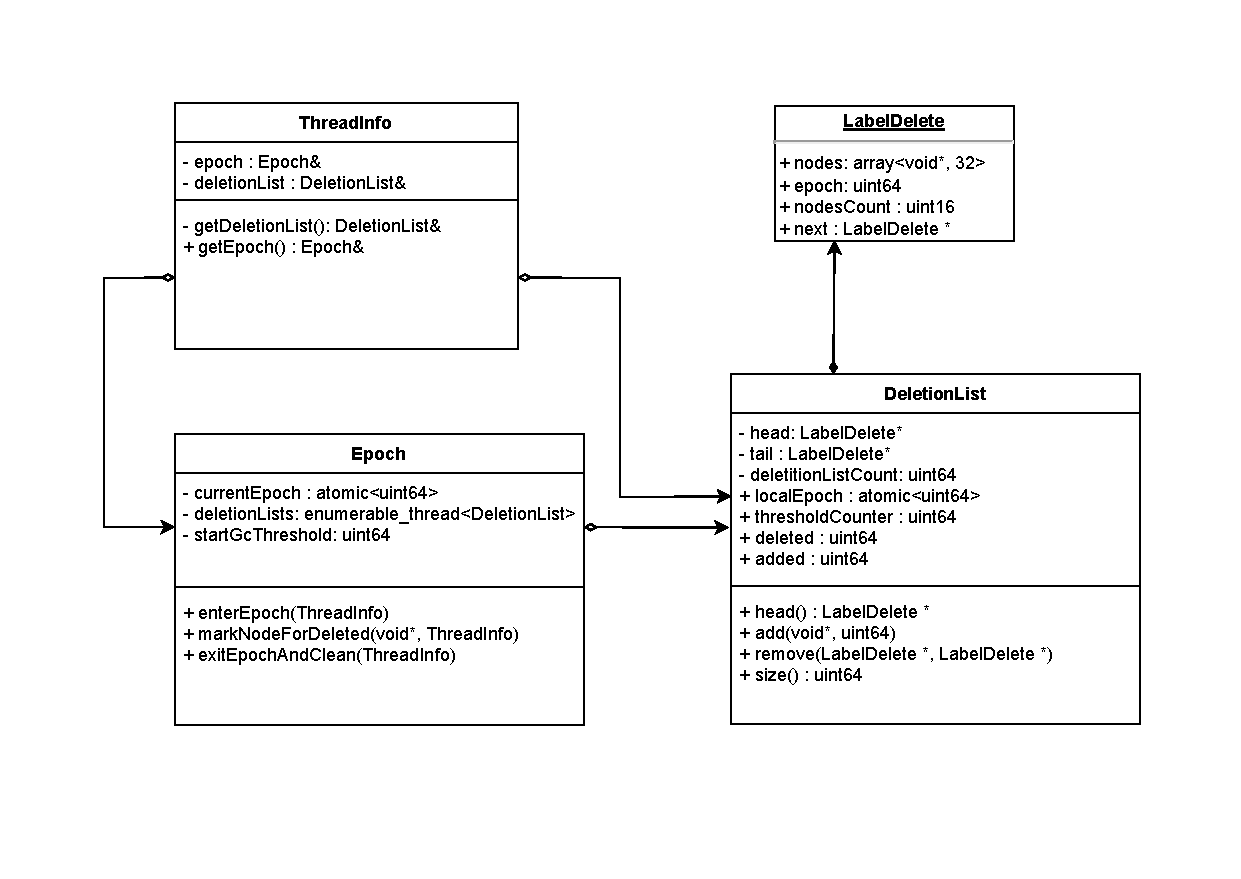
\includegraphics[width=1\textwidth]{art-epoch-gc.pdf}
  \caption{去中心化的垃圾回收类的类图}
  \label{fig:art-epoch-gc}
\end{figure}


两种内存管理机制分别是基于epoch的垃圾回收机制和基于无锁链表的垃圾回收机制。下图为基于epoch的垃圾回收的对象实现。
下面我们主要实现的是threadInfo类,epoch类。

对于epoch类,每个epoch会维护thread\_local的deleteList(被删除节点的链表),当前的epoch的信息以及一个垃圾删除的阈值
(低于该阈值的epoch上的标记删除节点可以真正的被回收),而threadInfo主要包含两个属性,分别是对epoch的引用和对待删除节点
列表的引用。

正常的流程如下,当某个工作线程T1需要对索引操作时,会根据当前索引中的epoch生成一个threadInfo .这里我们参考标准库中对mutex
的lock\_guard封装。采用RAII的思想,设计两个类EpocheGuard和EpocheGuardReadOnly
分别代表只读操作和读写操作需要对epoch和deletionList进行的操作,从而在使用上避免了直接对锁进行操作,减少了人为的死锁可能性。

对于epoch类,主要其三个主要的接口分别为enterEpoche(), markNodeForDeletion(), exitEpocheAndCleanup()

\begin{itemize}

\item enterEpoche(): 进入epoch,读取当前的epoch值

\item markNodeForDeletion(): 将节点标记删除,注册到deletionList中,待删除。这里的deletionList是threadLocal的,所以可以做到
线程间互不影响。

\item exitEpocheAndCleanup(): 退出当前的epoch,并根据此时需要删除的节点个数是否满足阈值要求,若达到要求则将其删除。
此处会遍历所有的deletionList,用到了intel提供的支持threadLocal的函数库,可以方便便利所有的threadlocal对象。

\end{itemize}

以上三个接口就可以完成去中心化的垃圾收集机制,由于需要依赖特定的函数库,因此可能在其他平台上并不适用,目前在x86平台上,这套
方案是比较稳妥且方便的。而且不会造成系统性能瓶颈。

对于不能够使用以上基于去中心化的垃圾回收机制的平台,此处还有一套基于无锁链表的垃圾回收机制。主要实现原理如下。
在索引模块中维护一个art\_obj\_pool对象,每次申请新的节点时都会向此对象申请内存,而如果需要删除某个节点,只需要将
删除的节点通过CAS插入链表的头部即可。

\begin{figure}[h]
  \centering
  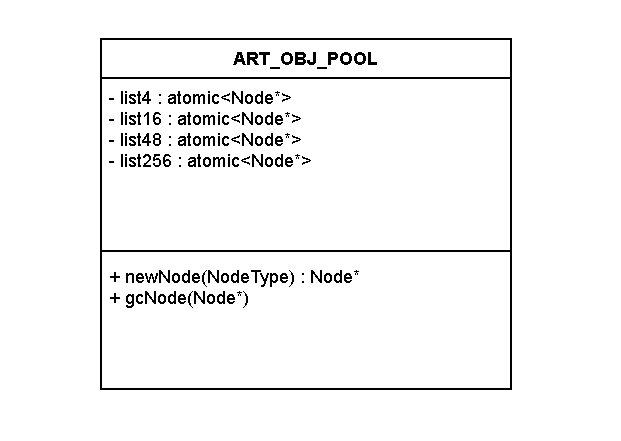
\includegraphics[width=0.9\textwidth]{art-obj-pool-class.pdf}
  \caption{无锁链表的垃圾回收类的类图}
  \label{fig:art-obj-pool-class}
\end{figure}

此方案有较大的改进空间,比如可以使用linux内核中常见的buddy内存分配算法,将小块的内存组合成大块,或者将大块的内存切分为
小块。
主要实现如下所示,当需要申请新的索引节点时,art\_obj\_pool会优先使用垃圾回收队列中的内存,根据申请的node类型,返回相应的
内存块,并在此基础上做初始化(placement new)。
这里有一点需要注意的是,对节点版本号应该继续加1,因为这里需要防止,节点刚刚被标记删除,随后就被回收,此时其他线程申请内存,
内存池返回该内存块,但是先前仍有其他内存持有该节点,此时,先前的线程认为节点可用,继续操作。因此我们在获得新的内存块时仍需要对其
版本号继续自增,这样先前的线程t2读取版本号发现已经变更,便会返回从根节点开始继续操作,而不会产生两个线程互相持有节点,导致节点操作异常。


\section{内存数据库表的组织方式}
结合以上的阐述,内存数据库中表的组织方式,目前数据库的表主要是以PAX方式进行组织。以4Mb为最基本的存储单位,每个block需要
做到4Mb字节的对齐。内存数据库中所有数据均存储在内存中,因此索引中的value只需要存储相应的记录的实际地址。针对PAX行列混存。
每个block内部的数据组织如下图。

\begin{figure}[h]
  \centering
  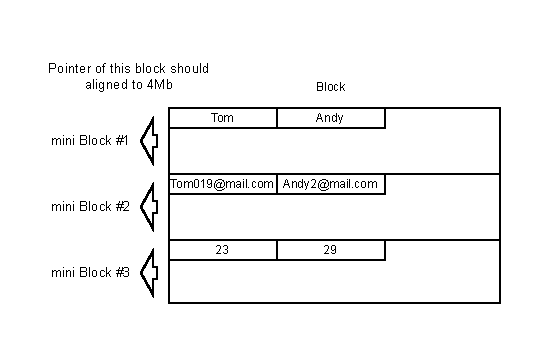
\includegraphics[width=0.9\textwidth]{PAX-class.pdf}
  \caption{PAX存储的内存布局}
  \label{fig:PAX-class}
\end{figure}

每个block内部数据按照列式存储,首先存储的是关于block的基本信息,其后为了实现上层事务中的MVCC事务并发控制。第一列存储对应
每一行的版本号指针,指向的是每一条undo log,实现多版本并发控制。其后存储的才是真正的数据。由于实际存储中可能会存在变长字段的
问题,解决这个问题可以引入一个全局的或者表级的变长字段管理器,所有变长字段可以作为一个长度为16字节的字段,如果长度小于8字节,
则直接存储在对应的block中,若长度大于8字节,则block中存储长度和地址,根据这两个参数到变长字段管理器,查询或者修改该字段的值。

索引中每一个叶子节点指向的都是版本号指针的地址,应用block头部的基本元信息,可以获取完整的一条记录。下图为block对外暴露的接口。
主要用于对表的修改,点查询,范围查询。

\begin{figure}[h]
  \centering
  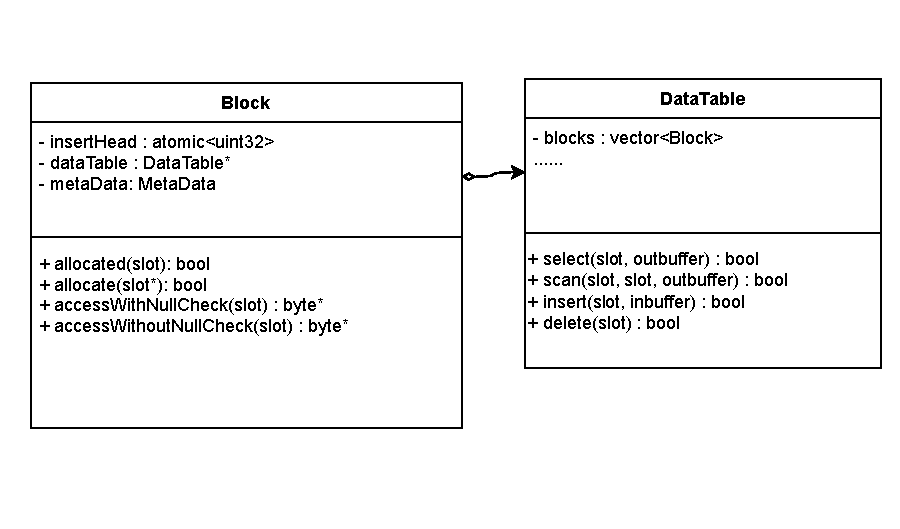
\includegraphics[width=0.9\textwidth]{PAX-class-2.pdf}
  \caption{PAX存储底层实现类的类图}
  \label{fig:PAX-class-2}
\end{figure}

\section{数据库索引的创建与管理的实现}

上述章节中详细介绍了数据库索引的结构,操作算法,内存管理,索引与表的联系,索引与事物的联系。作为本章的最后一个小节
将讨论索引最常规的操作就是create index 和drop index。本数据库中这两个操作都作为一个事务行操作,即允许其与其他DML操作
并发进行,而不会造成数据库一致性问题。

结合上文中提到的DAF模块,drop index的操作作为一个deferred action被注册到DAF Manager中。在这个deferred action中仍是一个
lambda表达式,表示这个动作还会被延迟执行。如下图所示。当前DAF Manager中有 drop index以及 对索引的插入操作。当daf执行
drop index时,会注册一个新的延迟操作到DAFmanager中,因此后面执行的对索引的插入操作仍然是可以进行的,不会造成插入一个空的
索引的问题。

而对于索引的生成则没有上述问题。索引创建主要是根据实际需要索引的字段创建相关的索引。根据之前章节所述的各种数据类型和索引key之间的
转换规则,如下,将实际的数据类型转换为索引中的key。作为keySchema传入indexBuilder,indexBuilder根据需要生成索引类型。
创建相关数据结构。并修改数据库系统中元数据。

以上是针对索引的创建和删除操作的实现,由于事务部分不是本片文章的重点,因此这里只是简单介绍一下关于如何处理索引的创建和删除过程
以下是一个完整的实现图。


\section{本章小结}

本章内容主要是从软件工程的角度,分析阐述如何实现具体的ART索引,以及基于乐观级联锁的方式处理对索引结构的并发操作。
分析了索引结构内存管理相关内容,以及如何将不同类型的数据组合成可以存储在索引中的键值数据。最后介绍了关于索引的DDL相关的
操作,简单描述DAF事务处理框架可以处理索引创建删除等操作,而不会引起任何内存或者其他一致性问题。